\chapter{Conclusion}

\section{Summary}

To summarise this thesis, the \gls*{mcrt} method is a powerful technique that can be used to calculate the transport of light (as particles or quasi-wave/particles) through turbid media, whilst modelling multiple anisotropic scattering alongside a variety of microphysics.
The only noted downsides to the \gls*{mcrt} method noted in the literature (as well as discussed at length in this thesis) is the computational load required for some problems, and the selection of optical properties.
With the growing power of computational devices, the computational load of \gls*{mcrt} becomes less of a factor.
Likewise the optical properties of various biological tissues, are increasing being measured with greater precision and accuracy.

\medskip

Chapter 1 introduced the concept at the heart of this thesis, the Monte Carlo method.
The chapter gave examples of how the Monte Carlo method can be used to sample from spectra, and how it is can be used to model various physical events.
Chapter 2 followed on from chapter 1's explanation of the Monte Carlo method, by introducing \gls*{mcrt} used in all subsequent chapters.
Chapter 2 also covered the theory behind the method and presented details of the implementation of the method into code as well as various computational speedups utilised.

\medskip

Chapter 3 described the application of the \gls*{mcrt} method to modelling tissue ablation.
Details of how the \gls*{mcrt} was coupled up to a numerical model of heat diffusion and thermal damage model was presented.
The chapter showed that we can successfully model experimental and theoretical data with our numerical model.
The power the model has is that we can predict thermal damage, and ablation crater size for any laser, and configuration thereof, without the need to test on humans or animals.
It also allows the testing of different lasers without the purchase of said laser, which could allow clinicians to ``try before they buy''.
The chapter also presented (with tongue firmly in cheek) the application of this numerical model to humane spy disposal.

\medskip

Chapter 4 presented the modification of the \gls*{mcrt} method, such that it would allow the modelling of the photon packets as quasi-wave/particle packets, in place of the usual particle model the \gls*{mcrt} method models.
This was achieved via a few small changes within the code, based upon well understood theoretical models namely the Fresnel-Huygens principle.
The method was thoroughly validated against several theoretical expressions.
The method was also validated against experimental results from collaborators at the University of Dundee.
The new method was then used to compare Bessel and Gaussian beams performance in highly turbid media, to see which beam preformed ``better''.
\medskip

Chapter 5 presented a model of skin autofluorescence using \gls*{mcrt}.
The chapter detailed a five layer skin model created to approximate the skin.
The five layer model included the various chromophores found in the skin such as blood, water, and melanin.
The model also includes various naturally occurring fluorophores.
Changes in the autofluorescent response of tissue has been shown to be indicative of various diseases.
However, details of how each fluorophore contributes to the signal is not well understood.
Therefore, a study on how tissue optics affects the autofluorescent signal, and how much each fluorophore contributes was undertaken.
The \gls*{mcrt} algorithm was also coupled to an optimisation technique to determine relative concentrations of the fluorophores in the skin from a given autofluorescent signal.
The technique chosen was the Nelder-Mead method.
The \gls*{nm} method uses simplices in order to move around the search space and find global minima.
The method was coupled to the MCRT algorithm and validated against toy models.
Finally details of how autofluorescent data from collaborators was fitted to using these techniques was presented.

\section{Future Prospects}

There are several avenues of promising work that can continue on from this thesis.

The code developed as part of the tissue ablation chapter, could easily be adapted for use in modelling photothermal therapy.
Photothermal therapy is the use of light to selectively heat up nanoscale materials that have been inserted into tumours.
The nanoscale materials, such as gold nanorods, are targeted with a specific wavelength of light (usually near infra-red) which heats up the rods and thus the surrounding tissue, eventually killing the adjacent cells~\cite{singh2016application,gallina2016aptamer}.
This could be easily modelled within the code developed as part of chapter 3, with little to no major changes.
The code could be used to help optimise photothermal treatment modalities and predict treatment outcomes.

There is also scope to improve the heat transfer model.
As mentioned in the chapter, a simple explict model was used as it relatively easy to setup and solve a given problem using this scheme.
However, this scheme leads to constraint on the timestep.
This could be avoided by using an implicit scheme which is unconditionally stable for any timestep.
Another way the heat transfer model could be improved is thought the use of the \gls*{fem}.
The \gls*{fem} allows PDEs to be solved on arbitrary grids, which would reduce the high memory requirement our model needs to achieve good resolution.
The \gls*{fem} would also allow a more accurate skin model to be included within the simulation, making the simulation more realistic.

Finally, the work of chapter 3 could also be extended to include a drug diffusion model.
One use of tissue ablation is a an optical drill to create micro holes in the skin. 
These holes in the skin then allow better penetration of topical drugs.
Modelling both the laser tissue ablation process and drug diffusion process in one simulation would allow \textit{in-silico} testing of treatment parameters which could easily be optimised by the model.

\medskip

The algorithm developed as part of chapter 4's work, $\varphi$MC, also has several avenues of future research.
It should be fairly easy to extend the algorithm to model other beams, such as an Airy beam.
It should also be fairly trivial to implement a spatial light modulator (SLM)\@.
An SLM is a device that can modulate light that is incident on it including imparting phase to different parts of the incident beam.
This allows arbitrary complex beams to be created.
The ability to model an SLM would open up the ability to model complex experiments in such things as wavefront shaping.
Other types of experiments the algorithm could be used for include: laser speckle imaging, focusing light though turbid media, and complex micromanipulation~\cite{vellekoop2007focusing,horstmeyer2015guidestar,vcivzmar2010situ}.

\medskip

One obvious avenue of future research would be to improve the five layer skin model presented as part of chapter 5's work.
The skin model presented is planar, where as tissue is not planar in any sense.
The first improvement on this could be to introduce a more complex geometrical structure into the voxel model.
However, this method would quickly run into a computational wall.
To represent the non planar reality of the tissue would require many voxels, such that the RAM required to run any simulation would be prohibitive to running the simulations.
Therefore, a different geometrical model would need to be used.
A solution to this was briefly investigated: use of a mesh to model the skin's structure.
Triangular meshes can be used to approximately model any arbitrary shape or volume.
The use of triangular meshes have been used to great effect by other authors in \gls*{mcrt} codes.
Due to time constraints this was abandoned for this thesis before a fully working code could be developed.
\Cref{fig:mesh} shows \gls*{mcrt} being preformed on a gourd made from a triangular mesh using the code developed as part of testing this method.

\begin{figure}[!htpb]
    \centering
    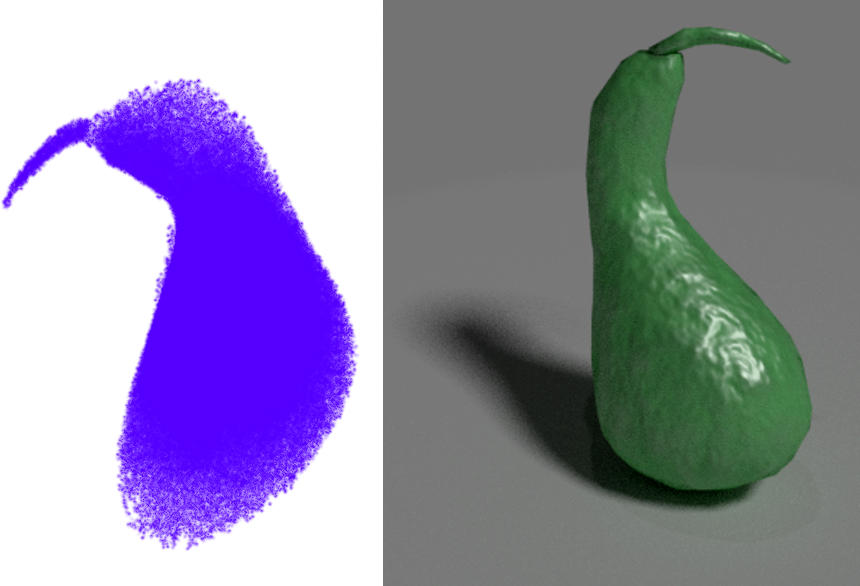
\includegraphics[width=0.5\textwidth]{gourd-fluence.png}
    \caption{Image on the left shows the fluence of light in a gourd, calculated using \gls*{mcrt}. The optical properties of the gourd in this simulations are similar to that of skin. The optical properties of the medium around the gourd are that of air. Image on the right shows a rendering of the same mesh in blender.}
    \label{fig:mesh}
\end{figure}

A meshed skin model would allow objects like hairs, blood vessels, sweat glands, and the uneven boundaries between skin layers greatly increasing the accuracy of the simulations.

Finally as the data from our collaborators equipment was not of a quality such that it could be reproduced using amoebaMCRT, this data could be taken again with a better equipment, or other authors could be found that have the requisite data. 
AmoebaMCRT would then be run on this data to determine the amount of that each fluorophore contributes to the signal.
Other optimisation techniques other than the \gls*{nm} method could also be explored.
Techniques such as simulated annealing, genetic algorithms\footnote{The use of genetic algorithms was explored, however the computational cost of using them was deemed too high.} or machine learning could be used.
It could also be possible for our \gls*{mcrt} code to be used to create a ``bank'' of spectra that could then be used to train a machine learning algorithm to label peaks, and contributions to those peaks by fluorophores.
